\begin{figure*}[tbp]
\centering
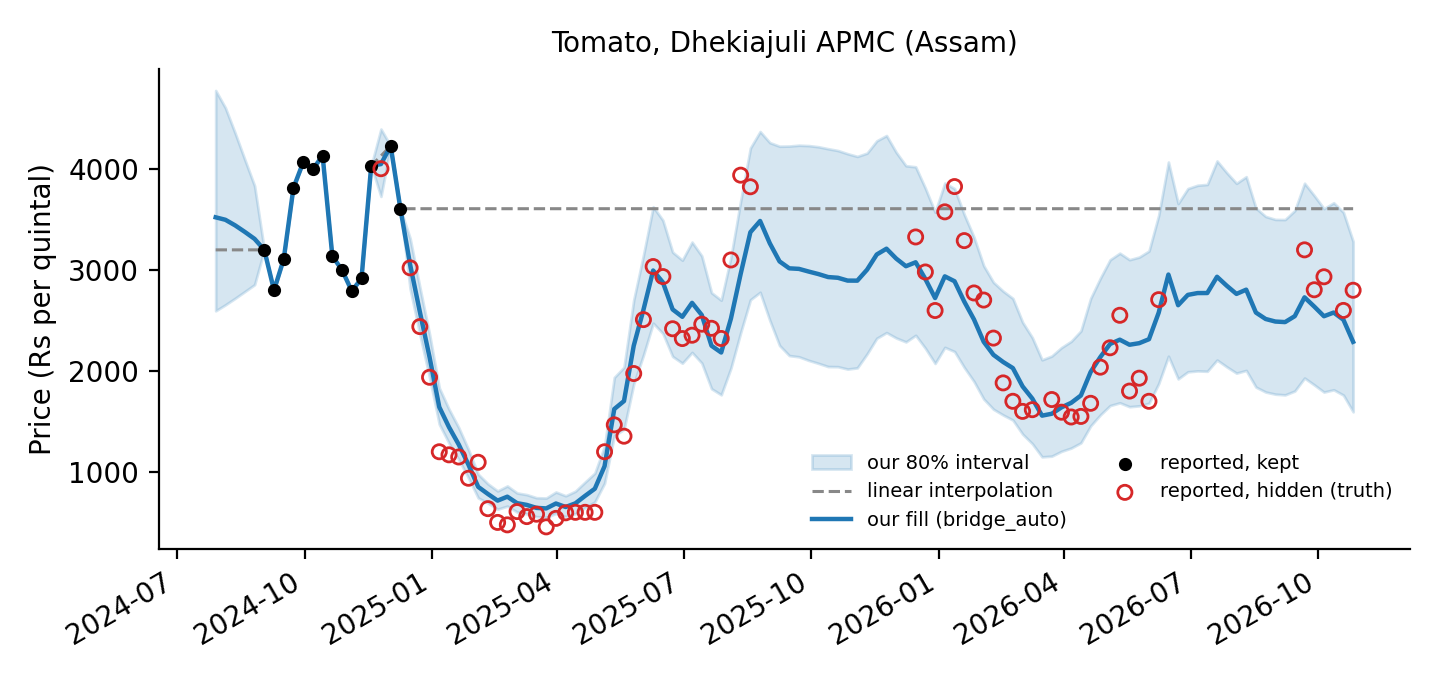
\includegraphics[width=0.84\textwidth]{fig_example.png}
\caption{Selected long-gap illustration for Tomato at Dhekiajuli APMC, Assam: retained reports, hidden real reports, the adaptive fill and nominal-80\% interval, and linear interpolation. Selection searched Potato, Tomato and Onion over twelve transplant seeds, preferring long gaps with at least fifteen hidden reports and more retained observations. This is an illustrative hard case, not a representative sample or evidence of calibrated uncertainty in original gaps.}
\Description{A selected tomato series shows a prolonged hidden interval where the adaptive estimate changes with the panel signal while linear interpolation remains nearly flat.}
\label{fig:example}
\end{figure*}
